% !TEX root = ../presentation.tex

\begin{frame}{Общий вид FCN}
\begin{figure}
\centering
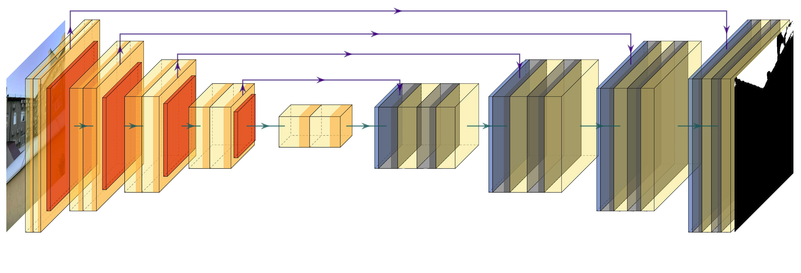
\includegraphics[width=9.01cm, height=3.73cm]{net_arch.png}
\end{figure}
    Энкодер и декодер части сети.
    Такой подход позволяет выделить признаки, а затем генерализировать их для классификации.
%\textbf{$C$}-центр камеры (оптический центр); \textbf{$Cp$}-главная ось камеры
\end{frame}